\documentclass[12pt]{exam}
	
\usepackage[margin=1in]{geometry}		% For setting margins
\usepackage{amsmath}				% For Math
\usepackage{amsfonts}
\usepackage{amssymb}
\usepackage{fancyhdr}				% For fancy header/footer
\usepackage{graphicx}				% For including figure/image
\usepackage{cancel}	
% To use the slash to cancel out stuff in work
\usepackage{wrapfig}
\usepackage{tikz}
\usepackage{float}
\usepackage{subfiles}
\usepackage{caption}
\usepackage{subcaption}
%%%%%%%%%%%%%%%%%%%%%%
% Set up fancy header/footer
\pagestyle{fancy}
\fancyhead[LO,L]{Kate O'Neill - 21365768}
\fancyhead[CO,C]{MAUC200 - Assignment 4}
\fancyhead[RO,R]{\today}
\fancyfoot[LO,L]{}
\fancyfoot[CO,C]{\thepage}
\fancyfoot[RO,R]{}
\renewcommand{\headrulewidth}{0.4pt}
\renewcommand{\footrulewidth}{0.4pt}
%%%%%%%%%%%%%%%%%%%%%%
\begin{document}
\begin{questions}
\question
\begin{parts}
\part 
\[y = \lceil x \rceil \Rightarrow y \in \mathbb{N}\] 
\[\Rightarrow (x,y) \in \mathbb{R} \times \mathbb{N}\] 
\(\{(x,y)\in \mathbb{R}^2 | y = \lceil x \rceil\}\) is a disjoint union of an uncountably infinite set \(\mathbb{R}\) and a countably infinite set \(\mathbb{N}\). \\
\(\therefore \{(x,y)\in \mathbb{R}^2 | y = \lceil x \rceil\}\) is uncountably infinite.
\part
\[A = \{(x,y)\in \mathbb{R}^2 | x^2 + y^2 < 16\} \cap \{(x,y)\in \mathbb{R}^2 | x^2 + y^2 > 9\}\]
When graphed, \(\{(x,y)\in \mathbb{R}^2 | x^2 + y^2 < 16\}\) is the inner area of a circle, and \(\{(x,y)\in \mathbb{R}^2 | x^2 + y^2 > 9\}\) is the area outside of a smaller circle, also with a radius of 0. \(A\), the intersection of the two is the area of the annulus between the two.\\
\(\therefore A\) is finite.
\part
An isomorphism between \((V,E)\) and \((V',E')\) is a bijective function between \(V\) and \(V'\) that preserves \(E\) and \(E'\).
\((V,E)\) is a complete graph, every vertex is adjacent to every other vertex\(\Rightarrow\) there are \(n!\) possible isomorphisms of the graph \((V,E)\) to itself.
\[\Rightarrow |A|=n!, n \in \mathbb{N}\]
\(\therefore\) \(A\) is finite.
\part
Assuming that \(\mathbb{P} (\mathbb{P} (\mathbb{Q}))\) is countable,\\
\(\mathbb{P}( \mathbb{P}( \mathbb{Q})) = \{S_1, S_2, S_3, \cdots\}\), where \(S_i\) is a subset of \(\mathbb{Q}\).
We cannot ensure that every subset is enumerated.\\
\(\therefore \mathbb{P} (\mathbb{P} (\mathbb{Q}))\) is uncountably infinite.
\part
According to the lectures, any regular expression is either finite or countably infinite, and we must see which statement holds in this case. \\
\(\emptyset *\) and \(\epsilon *\) are finite.
\((A \circ A \circ A)\) is an uncountably infinite set.
\(\therefore A\) is uncountably infinite.
\part
All regular expressions are either finite or countably uncountably infinite, according to the lectures.
\(\therefore L_{REX}\) is countably infinite.
\end{parts}
\question
\begin{parts}
\part
\begin{enumerate}
    \item Begin at the leftmost cell.
    \item If the current cell contains any symbol other than \(a, l, p\), REJECT.
    \item If the current cell contains \(a\), delete it, and move right to the next cell. Go to step 2.
    \item If the current cell contains p, move right to the next cell and go to step 8.
    \item If the current cell contains\(l\), move right to the next cell.
    \item If the current cell contains \(a\), ACCEPT.
    \item Go to step 2.
    \item If the current cell contains \(l\), ACCEPT.
    \item Go to step 2.
\end{enumerate}
\begin{itemize}
    \item \(aaa: \underline{a}aa \rightarrow \_\underline{a}a \rightarrow \_\_\underline{a} \rightarrow \) REJECTED
    \item \(lal: \underline{l}al \rightarrow l\underline{a}l \rightarrow\) ACCEPTED
    \item \(pplap: \underline{p}plap \rightarrow p\underline{p}lap \rightarrow pp\underline{l}ap \rightarrow ppl\underline{a}p \rightarrow\) ACCEPTED
\end{itemize}
\part
\begin{figure}[H]
    \centering
    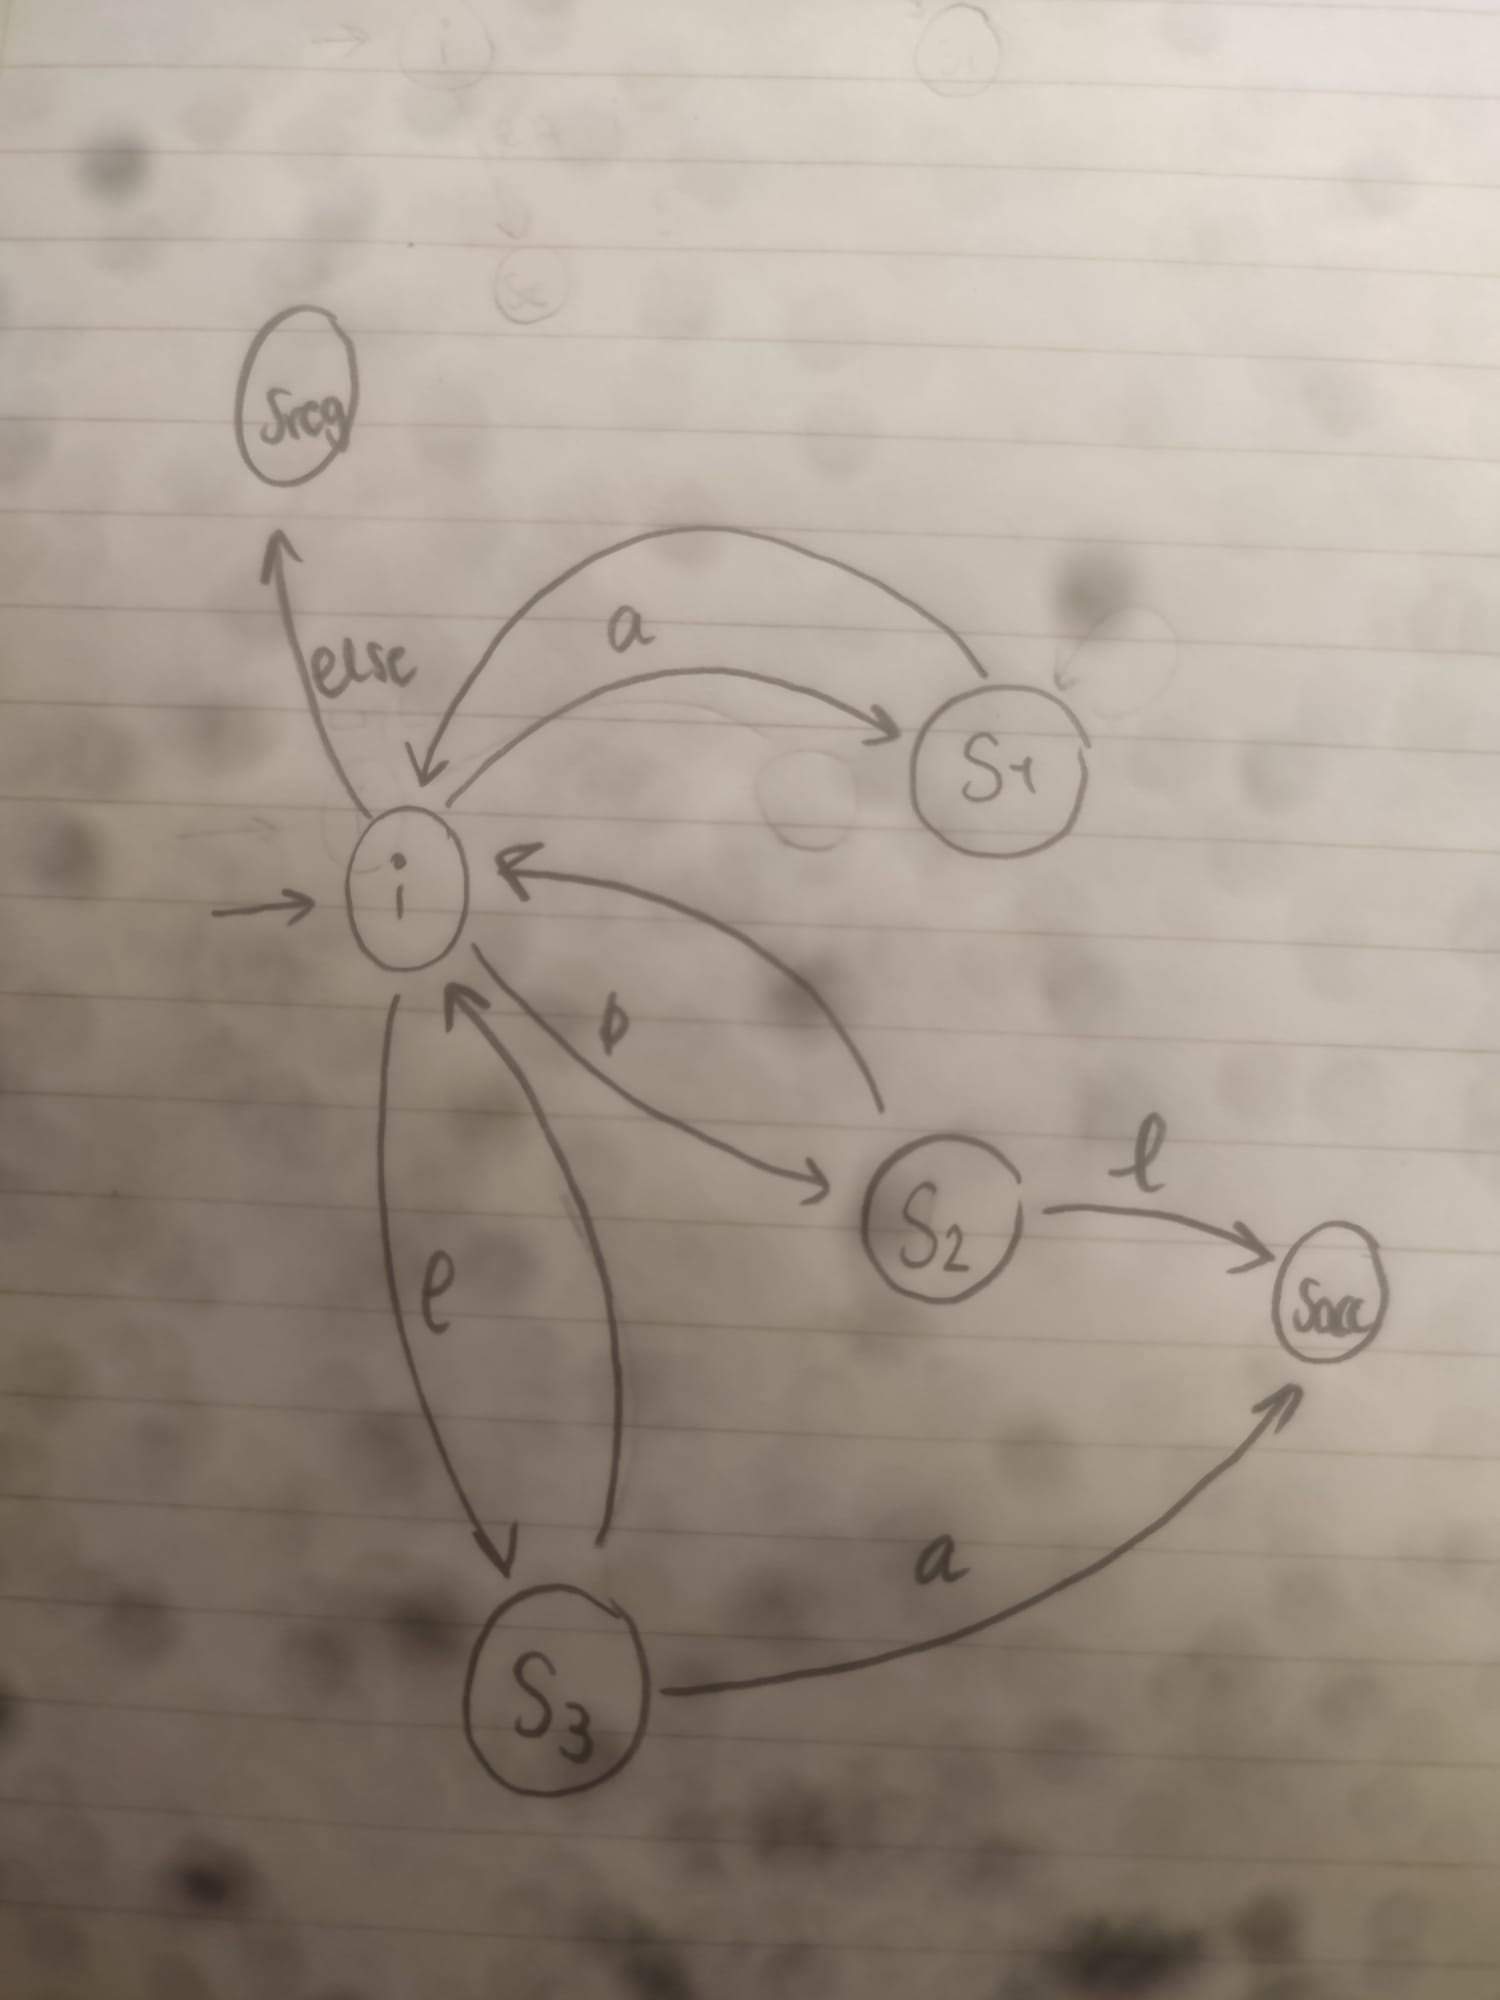
\includegraphics[scale=0.2]{turingmhcine.jpeg}
\end{figure}
\end{parts}
\question
In order prove this, we need to show that the union or intersection of two Turing-recognisable languages is also Turing-recognisable.\\
Let \(L_1, L_2\) be Turing-recognisable languages. We must construct a Turing machine that recognizes \(L_1 \cup L_2\), and another one that recognizes \(L_1 \cap L_2\).

\end{questions}
\end{document}